\documentclass[12pt]{report}
\usepackage{listings}
\usepackage{xcolor}


            \lstset{
            tabsize = 4, %% set tab space width
            showstringspaces = false, %% prevent space marking in strings, string is defined as the text that is generally printed directly to the console
            numbers = left, %% display line numbers on the left
            commentstyle = \color{blue}, %% set comment color
            keywordstyle = \color{orange}, %% set keyword color
            stringstyle = \color{green}, %% set string color
            rulecolor = \color{black}, %% set frame color to avoid being affected by text color
            basicstyle = \small \ttfamily , %% set listing font and size
            breaklines = true, %% enable line breaking
            numberstyle = \tiny,
        }


\usepackage[french]{babel}
\usepackage[T1]{fontenc}
\usepackage[utf8]{inputenc}
\usepackage[final]{pdfpages} 
\usepackage{titlesec}
\usepackage{setspace}
\usepackage{color}
\usepackage[nottoc, notlof, notlot]{tocbibind}
\usepackage{hyperref}
\usepackage{float}
%\usepackage{slashbox}
\usepackage{diagbox}
\usepackage{biblatex}
\usepackage{listings}
\usepackage{lscape}
\usepackage{geometry}
\usepackage{geometry}
 \geometry{
 a4paper,
 total={170mm,257mm},
 left=20mm,
 top=20mm,
 }
\bibliography{Bibliographie.bib}

\titleformat{\chapter}{\bf\huge}{\thechapter}{0pc}{}
\begin{document}

\begin{titlepage}
\begin{center}

% Upper part of the page. The '~' is needed because only works if a paragraph has started.

\includegraphics[width=0.8 \textwidth]{images/univ.jpg}\\[1cm]

{\scshape\LARGE PROJET DE FIN D'ÉTUDES\par}

	\vspace{2cm}

\textsc{\LARGE  Master 2 Informatique}\\[1.5cm]

\textsc{\Large }\\[0.5cm]
{\huge \bfseries EVERNET - TRANMISSION DE SLOTS ET NETWORK CODING\\
	\vspace{1.5cm}
RAPPORT \\[0.2cm] }

	\vspace{3cm}	
% Author and supervisor
\begin{minipage}{0.4\textwidth}
\begin{flushleft} \large
\emph{Auteurs}\\
BALLION Lucas  \\
DIALLO Abdoul  \\ 
DIALLO Thierno   \\
HOARAU Raphael   \\
PORTEJOIE Sarah \\
KARA Zoubir  
\end{flushleft}
\end{minipage}
\begin{minipage}{0.4\textwidth}
\begin{flushright} \large
\emph{Client} \\
Serge  \textsc{CHAUMETTE}\\
\emph{Référent} \\
Pascal \textsc{DESBARATS}
\end{flushright}
\end{minipage}
	
\vfill

% Bottom of the page
{\large \today}

\end{center}
\end{titlepage}

\tableofcontents
\listoffigures

\include{introduction}
\chapter{ ANALYSE DE L'EXISTANT}

Plusieurs applications pour téléphone mobile, permettant l'envoi de messages et/ou d'images, sont déjà disponibles sur le marché. Parmi celles-ci, on retrouve notamment WhatsApp, Telegram et Signal.\\
\begin{itemize}
    \item  WhatsApp permet l'envoi de messages et d'images en utilisant une connexion internet fixe ou par un réseau internet mobile (3G,4G). Elle offre un chiffrage de bout en bout des communications et compte plus de 2 milliards d'utilisateurs à travers le monde.\\
    Bien que les communications soient chiffrées, WhatsApp fait face à des critiques concernant la confidentialité des données personnelles échangées sur la plateforme. \\
    Cela notamment depuis son rachat en 2014 par Facebook et la mise en place de nouvelles conditions d'utilisations début 2021. Conditions qu'il est obligatoire d'accepter afin de continuer à utiliser le service. 
    \\Ceci a eu pour conséquence, de provoquer une fuite d'un certain nombre d'utilisateurs vers des services concurrents.\\
    
    \item Telegram est une application de messagerie permettant d'échanger des messages et des documents de manière sécurisée. 
    \\La partie cliente est libre alors que la partie serveur est propriétaire. A l'origine, l'application a été développée par deux frères russes Nikolaï et Pavel Dourov afin de pouvoir communiquer tout en évitant la censure. 
    \\Certains experts en sécurité émettent des doutes sur le mode d'authentification de Telegram. Ils expliquent qu'il serait possible d'usurper l'identité d'un utilisateur en interceptant le code SMS de vérification. 
    \\Actuellement l'application compte plus de 500 millions d'utilisateurs à travers le monde.\\
    
    \item Signal est une application conçue dans le but d'être la plus sécurisée possible. Elle réalise une collecte minime des données personnelles des utilisateurs. Sa distribution est sous licence libre. 
    \\Elle est financée par la Signal Foundation qui est une association à but non lucratif. Son haut niveau de sécurité fait qu'elle est recommandée par des personnalités comme Edward Snowden ou Elon Musk. La commission européenne recommande à son personnel l'utilisation de Signal. 
    \\Moins utilisée que ses concurrents, signal connaît un certain succès, notamment depuis le changement des conditions d'utilisation de WhatsApp, qui entraîna 47 millions de téléchargements en deux semaines pour Signal.\\
    
\end{itemize}
\paragraph{}L'application Evernet offre un protocole d'échange d'image sécurisé. Sa principale différence vis à vis des solutions existantes est le fait qu'elle n'utilise que les SMS pour l'envoi de fichiers. L'autre particularité d'Evernet contrairement aux autres solutions disponibles, est qu'elle permet uniquement l'échange d'image et non de messages et autres types de documents.

\paragraph{}Le Network Coding est un thème de recherche qui a été récurant à la fin des années 90 et au début des années 2000. Son objectif est d'améliorer le débit, l'efficacité et l'évolutivité d'un réseau de communication. 
\\Un autre avantage du Network Coding est qu'il permet d'augmenter la résistance du réseau aux attaques. Son principe de base consiste à faire transiter sur un lien de communication plus d'un paquet à la fois. Lorsqu'un noeud du réseau reçoit deux paquets celui-ci va agréger les deux paquet de manière à ne faire circuler sur le lien qu'un seul paquet. Pour parvenir à cela, une opération binaire (par exemple un XOR) va être faite sur le payload des deux paquets pour ne constituer qu'un seul paquet. On peut donc faire transiter sur un seul lien plus de données dans la même unité de temps et on accroît donc le débit du réseau, de plus, le codage appliqué au payload va permettre de renforcer la sécurité globale du réseau. L'utilisation de ce protocole dans notre projet va permettre d'améliorer les performances globales du réseau ainsi que sa sécurité.    


\chapter{ ANALYSE DES BESOINS}

\section{Les besoins fonctionnels}

        \subsection{Communication avec le serveur}
        Pour éviter toute intrusion d'une personne extérieure et garantir la sécurité des utilisateurs, un serveur a été mis en place par le groupe 1. Ce dernier garantit la vérification de l'identité des utilisateurs, donc tout utilisateur doit pour faire partie du réseau disposer d'une invitation valide qui va lui permettre de s'inscrire.  Ce serveur enregistre tous les utilisateurs, il contient donc les pseudonymes, les numéros de téléphones et les certificats.
        Notre application communique avec ce serveur lors de l'inscription d'un utilisateur(utilisation d'un lien d'inscription valide), lorsque ce dernier souhaite se connecter à l'application(vérification de l'adéquation pseudonyme et mot de passe) mais aussi quand il souhaite envoyer une image à un autre utilisateur(récupérer une liste de numéros par lesquelles doivent transiter les paquets).
            
        
        \subsection{Authentification}
        Lors de son inscription, un utilisateur doit fournir son numéro de téléphone, choisir un identifiant et un mot de passe. La page d'accueil de l'application offre donc une interface pour permettre l'enregistrement de ces informations.
        Lors de la première demande de connexion, une communication est établie avec le serveur pour vérifier les informations de l'utilisateur afin de lui permettre d'accéder aux services fournis par l'application.
        
        \subsection{Ajouter un contact}
        Une fois connecté, comme dans tout réseau social, on a souvent des échanges et des interactions avec les mêmes personnes. Donc pour faciliter les communications entre les utilisateurs, un service d'ajout de contact a été implémenté. Ainsi tout utilisateur peut ajouter des contacts et donc avoir une liste d'amis avec lesquels interagir. Lors de l'envoi d'une image à un ami cette fonctionnalité n'empêche pas que les paquets sur le réseau transitent par les téléphones d'autres utilisateurs (authentifiés par le serveur) qu'on ne connaîtrait pas. Pour enregistrer un contact il faut fournir un nom et son identifiant.
        

        \subsection{Sélection d'un destinataire}
        
        Lorsqu'un utilisateur veut envoyer une image à un autre, il peut sélectionner ce dernier dans sa liste de contacts enregistrés.
       
        
        
        \subsection{Sélection de l'image à envoyer}
        Depuis la page d'envoi, l'utilisateur sélectionne l'image à envoyer dans la galerie d'images de son téléphone  en cliquant sur un bouton prévu à cet effet. %%indexer ici la capture d'ecran de la page d'envoie 
        
        Pour cela, l'utilisateur doit au préalable autoriser l'application à accéder à l'espace de stockage des images de son téléphone.
        
        \subsection{Envoi de l'image}
        Pour optimiser la taille des paquets, après avoir cliqué sur le bouton d'envoi, l'image sélectionnée est d'abord compressée, ce qui permet de faciliter son découpage en fragment d'images (voir ~\ref{decoupage} ). Chaque fragment est concaténé à d'autres champs pour former l'entête du paquet SMS(~\ref{epSMS}),  puis envoyé à des noeuds intermédiaires, qui à leurs tours le renvoient à d'autres, ainsi de suite. Le paquet se promène jusqu'à ce qu'il arrive à destination ou jusqu'à ce que son temps de vie (TTL: time to live) expire.
        
       
        %\subsection{Gestion de l'équilibre carbone}
        %pas gérée pour le moment
            

\section{Les besoins non fonctionnels}
        
        \subsection{Portabilité sur les différentes versions d'Android}
            L'application développée est compatible avec un maximum de terminaux android. Nous avons donc choisi une version minimale requise d'android permettant la plus large compatibilité possible. Il apparaît que rendre l'application compatible avec les systèmes android 4.4 et ses versions ultérieures, permet à environ 98\%
            des terminaux android sur le marché, d'être compatible avec notre application, ce qui est nettement suffisant. Notre application est donc compatible avec les systèmes android 4.4 et ultérieur.

        
        \subsection{Compatibilité avec les autres parties du projet global}
            Le projet Evernet étant divisé en trois sous-projets, notre application est en mesure de s'intégrer avec les deux autres sous-projets afin que le projet global puisse être fonctionnel. Elle est donc en capacité d'utiliser les services de sécurité offerts par le serveur fourni par le groupe 1. Le groupe 3 devant retracer le parcours des paquets sur le réseau, notre entête contient suffisamment d'informations afin que ceci soit possible. Des informations comme la source initiale, la destination finale sont indispensables au groupe 3 et sont donc présentes dans l'entête de nos paquets.  
        
        \subsection{Simplicité d'utilisation}
            
            La simplicité d'utilisation est essentiel pour l'expérience utilisateur. Une interface simple et ergonomique est nécessaire au bon développement de l'application. Une interface trop complexe conduira à une non-utilisation de l'application par les publics cibles qui se tourneront vers des solutions plus simples. Pour ce faire un respect des règles d'Interface Homme-Machine est nécessaire. Ces règles posent un cadre qui permet au développeur de réaliser l'interface la plus ergonomique et simple possible, pour que l'application soit plus simple et agréable à utiliser.
            
              \subsection{Environnement de développement}
            L'application est conçue pour fonctionner sous le système d'exploitation mobile android. Ce qui nécessite d'utiliser un environnement de développement approprié.
            Il a donc été choisi d'utiliser Android Studio. 
            
            \subsection{Langage de programmation}
            Java est le langage de programmation qui a été retenu pour ce projet. Ce dernier étant recommandé par le client, est compatible avec Android Studio. Le langage Kotlin est également compatible avec Android Studio. Seul Java est connu par tous les membres de notre groupe.
\section{Contraintes}
Ce projet amène différentes contraintes techniques qui sont :
\\

\begin{itemize}
\item [•]{Application du Network coding}
            
            La pierre angulaire de ce projet est l'utilisation du \textbf{Network Coding}. Cette façon de gérer les paquets SMS circulant sur le réseau permet d'optimiser le trafic, et d'augmenter la sécurité.
            Lorsque plusieurs paquets ayant la même destination arrivent sur un noeud du réseau, les données que ces paquets portent sont combinées pour former une seule donnée. On peut ainsi envoyer un seul paquet contenant les données combinées et la façon dont les données sont combinées.
            On réduit ainsi le nombre de paquets nécessaires pour transmettre l'information, on allège donc la charge sur le réseau.
            De plus la combinaison des données améliore la sécurité du réseau en chiffrant les données. La manière de combiner les données induit un chiffrement de ces données. On doit donc disposer de la formule de combinaison et d'un ou plusieurs paquets propres à chaque combinaison pour pouvoir déchiffrer les données.
            
            \begin{figure}[H]
                \centering
                
\includegraphics[scale=0.15]{images/Butterfly_network.svg.png}
                \caption{Exemple de Network Coding}
                \label{fig:exemple_Network_Coding}
            \end{figure}
            
            Comme on le voit ci-dessus, les paquets \textbf{A} et \textbf{B} sont combinés pour former un paquet \textbf{A}+\textbf{B}. Ce paquet \textbf{A}+\textbf{B} n'est déchiffrable dans ce cas-ci, seulement si on dispose du paquet \textbf{A} ou du paquet \textbf{B}.
            On retrouvera par exemple le paquet \textbf{B} en faisant : \\ (\textbf{A}+\textbf{B}) - \textbf{A} = \textbf{B}.
            \\
            
    \item [•] Absence de connectivité Internet :
    \\
    le système n'utilisera que les SMS
    \\
    
    \item [•] Equilibrage de la charge énergétique et de l'empreinte carbone :
    \\
    les différents slots de l'image passeront par différents mobiles intermédiaires
    de membres du réseau social
    \\
    
    \item [•]  Confidentialité :
    \\
     les numéros de mobiles des participants doivent rester confidentiels.
     Un serveur central est donc utilisé pour gérer l'association
     pseudonyme-numéro
     \\
     \item [•] Environnement non sécurisé avec risques de perte de messages
        et d'injection de faux messages :
        \\
        une PKI est mise en place pour assurer l'authentification des participants
     \\
     
     \item [•] Optimisation de la bande passante :
     \\
    la technique du Network Coding sera utilisée

\end{itemize}

\chapter{ ARCHITECTURE }

Nous avons choisi une architecture dites "MVC", Modèle, Vue, Contrôleur. 
Ce choix a été fait dans un but de maintenabilité. En effet notre projet, et plus particulièrement le dépôt Github du projet est partagé avec le groupe 3. Notre code étant donc repris par d'autres développeurs, il est nécessaire que celui-ci soit clair et bien organisé pour leur permettre de modifier ou d'ajouter des fonctionnalités.
\\
\begin{figure}[H]
    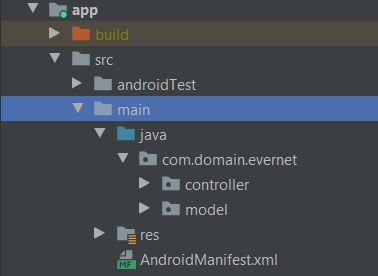
\includegraphics[width=10cm]{images/arbo.png}
    \caption{Arborescence de l'application Evernet.}
\end{figure}

\begin{itemize}
    \item [•] Modèle : \\
    Contient toutes les classes métiers nous permettant de traiter les données, ainsi que les communications.
    Cela inclut donc la communication avec le serveur central via Socket, les communications entre clients via SMS; la création de paquets; ainsi que le traitement des images. Ces fichiers sont accessibles dans le dossier model.
    \\
    
    \item [•] Vue \\
    Il s'agit ici de tous les fichiers XML permettant de construire l'interface utilisateur. Ces fichiers sont accessibles depuis le dossier res, les fichiers moteurs sont dans le dossier layout.
    \\
    
    \item [•] Contrôleur \\
    Cette partie contient toutes les classes activité et fragment qui permettent de faire le lien entre la vue et le modèle. La classe principale contrôlant le projet est MainActivity.
    Ces fichiers sont accessibles depuis le dossier controller.
    
\end{itemize}

\begin{figure}[H]
    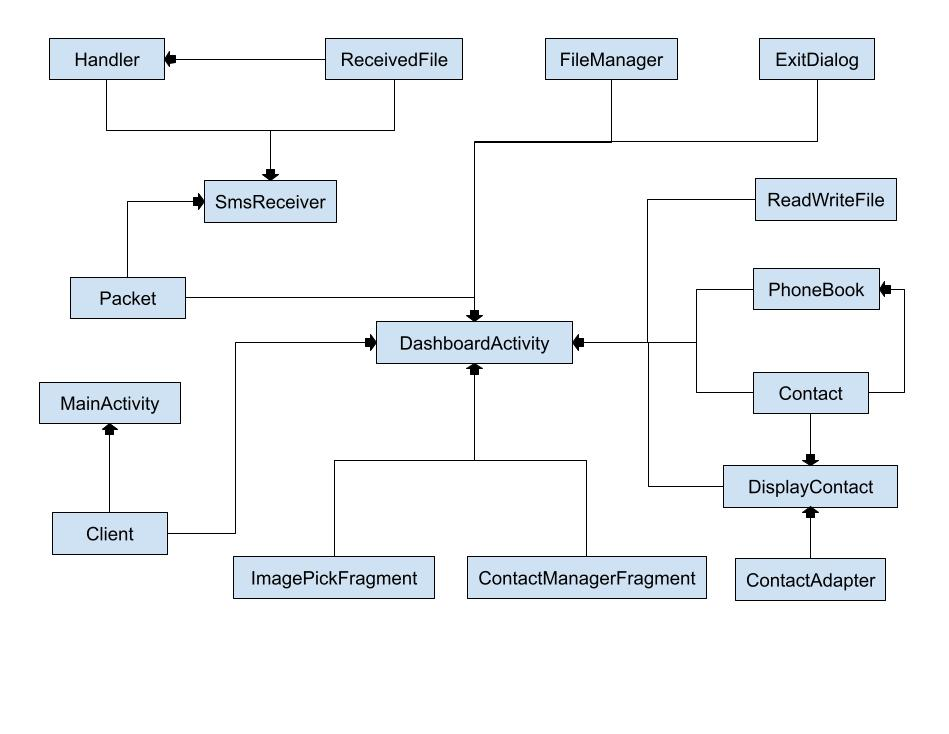
\includegraphics[width=15cm]{images/architecture.jpg}
    \caption{Diagramme de l'architecture.}
\end{figure}

\chapter{ GANTT PRÉVISIONNEL}

Le diagramme de Gantt est un outil de planification très utile voire même indispensable dans la gestion d'un projet informatique. Il permet de visualiser les différentes tâches d'un projet et leur niveau d'avancement ce qui améliore considérablement l'organisation et la gestion du temps disponible pour respecter les délais fixés pour la livraison d'un produit final au client. C'est donc tout naturellement, après la réception du sujet et nos divers échanges avec le client qu'on a établi le diagramme prévisionnel ci-dessous. Ce diagramme tient donc étroitement compte de notre compréhension initiale du sujet et des tâches indispensables identifiées pour le réaliser. 

\begin{figure}[H]
    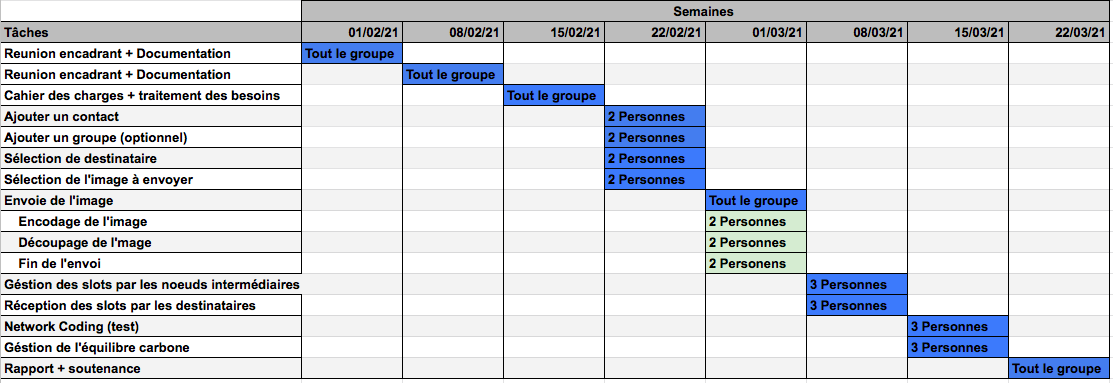
\includegraphics[width=18cm]{images/gantt.png}
    \caption{Gantt prévisionnel.}
\end{figure}

Très vite, après le début du projet, lors de nos rencontres hebdomadaires avec le client et les autres groupes impliqués dans ce projet, nous nous sommes rendus compte que les tâches succinctes qu'on avait identifiées au préalable seront amenées à évoluer/changer. C'est donc naturellement au fur des semaines qu'on a amélioré notre diagramme pour le mettre en adéquation avec l'avancement du projet. 

\begin{figure}[H]
    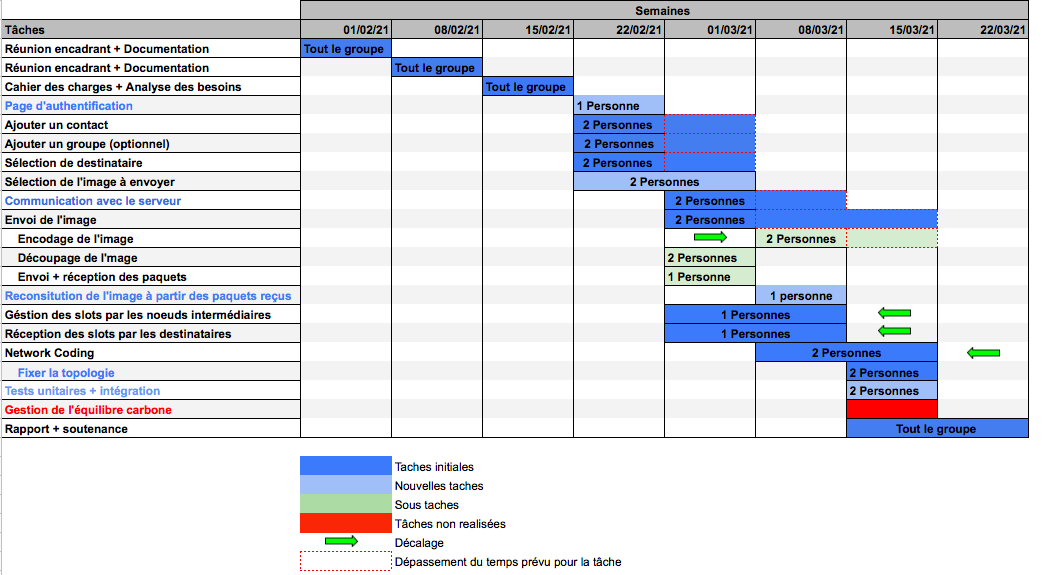
\includegraphics[width=18.5cm]{images/gantbis.png}
    \caption{Gantt effectif.}
\end{figure}

Identifier les tâches à effectuer est une chose relativement accessible, mais quantifier le temps de travail nécessaire pour la réalisation de certaines tâches demande de l'expérience dans la réalisation de ces dernières. Nous avons réussi à respecter les délais prévus durant le premier mois, mais on a dû adapter beaucoup de tâches dans la réalisation de la seconde partie du projet. 




\chapter{ USER STORY}


\section{Page d'authentification}
Les captures d'écran ci-dessous montrent l'interface graphique intuitive et facile à utiliser que nous avons mise en place. Au lancement de l'application, l'utilisateur tombe sur une fenêtre d'authentification où il doit renseigner son numéro de téléphone, son pseudonyme et son mot de passe. Les informations saisies par l'utilisateur sont vérifiées. Le numéro de téléphone ne doit comprendre que 10 caractères qui sont obligatoirement tous des chiffres de 0 à 9. Le pseudo de l'utilisateur est également vérifié, celui-ci ne doit pas comporter de caractère étoile "*" et de plus sa taille ne peut excéder 9 caractères. Une fois ces informations saisies mais aussi vérifiées et que l'utilisateur est authentifié auprès du serveur, cette page ne sera plus affichée, au lancement de l'application l'utilisateur sera directement redirigé vers la page principale de l'application. 
    \begin{figure}[H]
    \begin{center}
    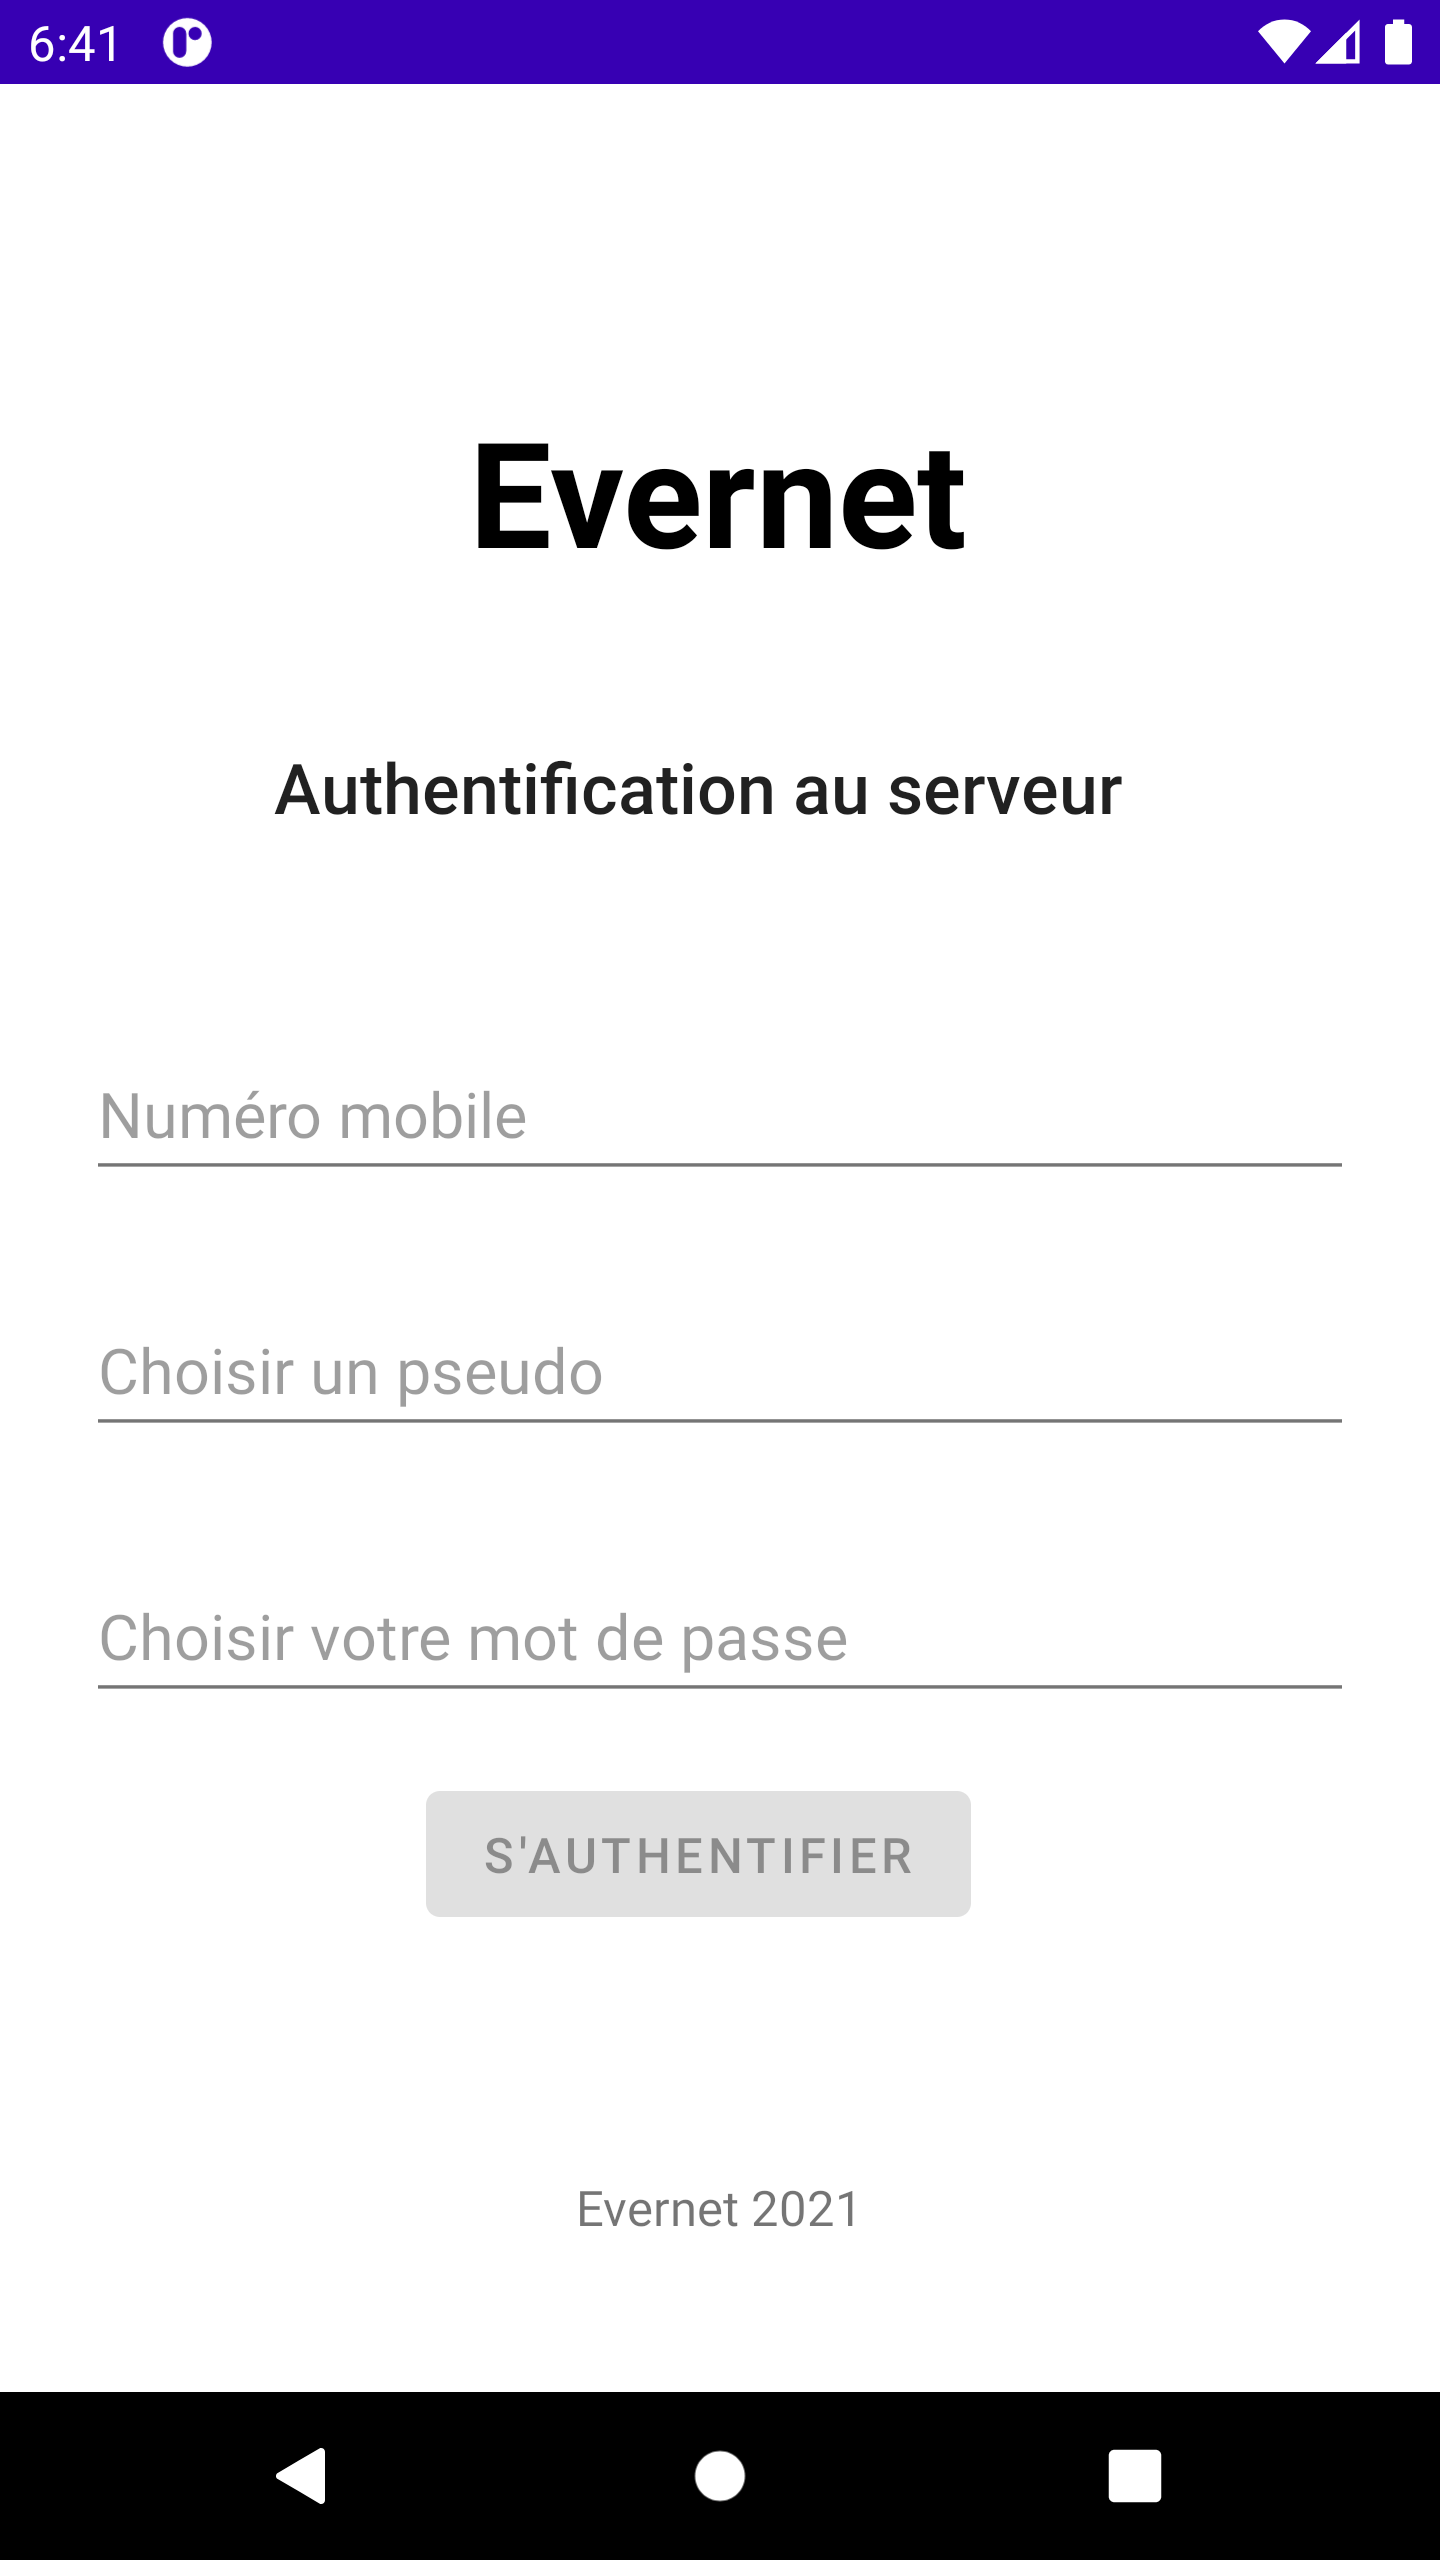
\includegraphics[width=7cm]{images/auth.png}
    \caption{Page d'authentification de l'application.}
    \end{center}
    \end{figure}
    
\section{Page principale}    
Après l'authentification, l'utilisateur arrive sur la page principale de l'application. Celle-ci comporte trois boutons, celui pour aller dans la page d'ajout des contacts, celui pour accéder au menu permettant l'envoi d'une image, ainsi qu'un bouton pour quitter l'application. Par défaut le menu permettant l'envoi d'une image est directement affiché. Celui-ci offre à l'utilisateur la possibilité de choisir une image à envoyer dans sa galerie, de choisir un destinataire parmi sa liste de contact et d'envoyer une image. Une fois l'image à envoyer sélectionnée, celle-ci apparaît dans le cadre d'image encore vide au lancement de l'application.
 
    \begin{figure}[H]
    \begin{center}
    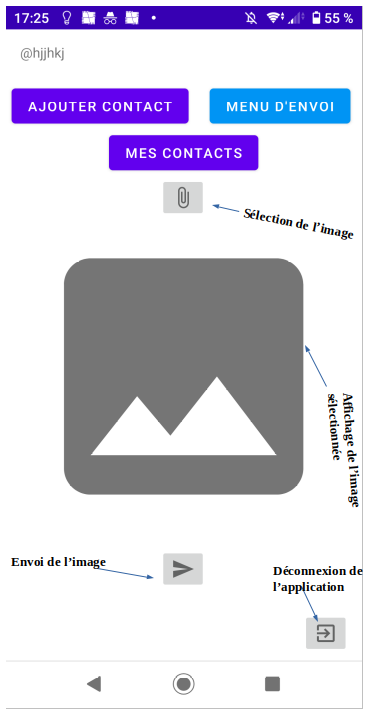
\includegraphics[width=7cm]{images/send_picture.png}
    \caption{Page d'accueil de l'application.}
    \end{center}
    \end{figure}
    

En appuyant sur le bouton "Mes contacts", l'utilisateur va voir apparaître une nouvelle page regroupant l'ensemble des contacts enregistrés sur l'application. Ceux-ci sont affichés sous forme de liste comportant le pseudo de l'utilisateur et en dessous de celui-ci l'id associé a cet utilisateur précédé d'un '\#'.    
\begin{figure}[H]
    \begin{center}
    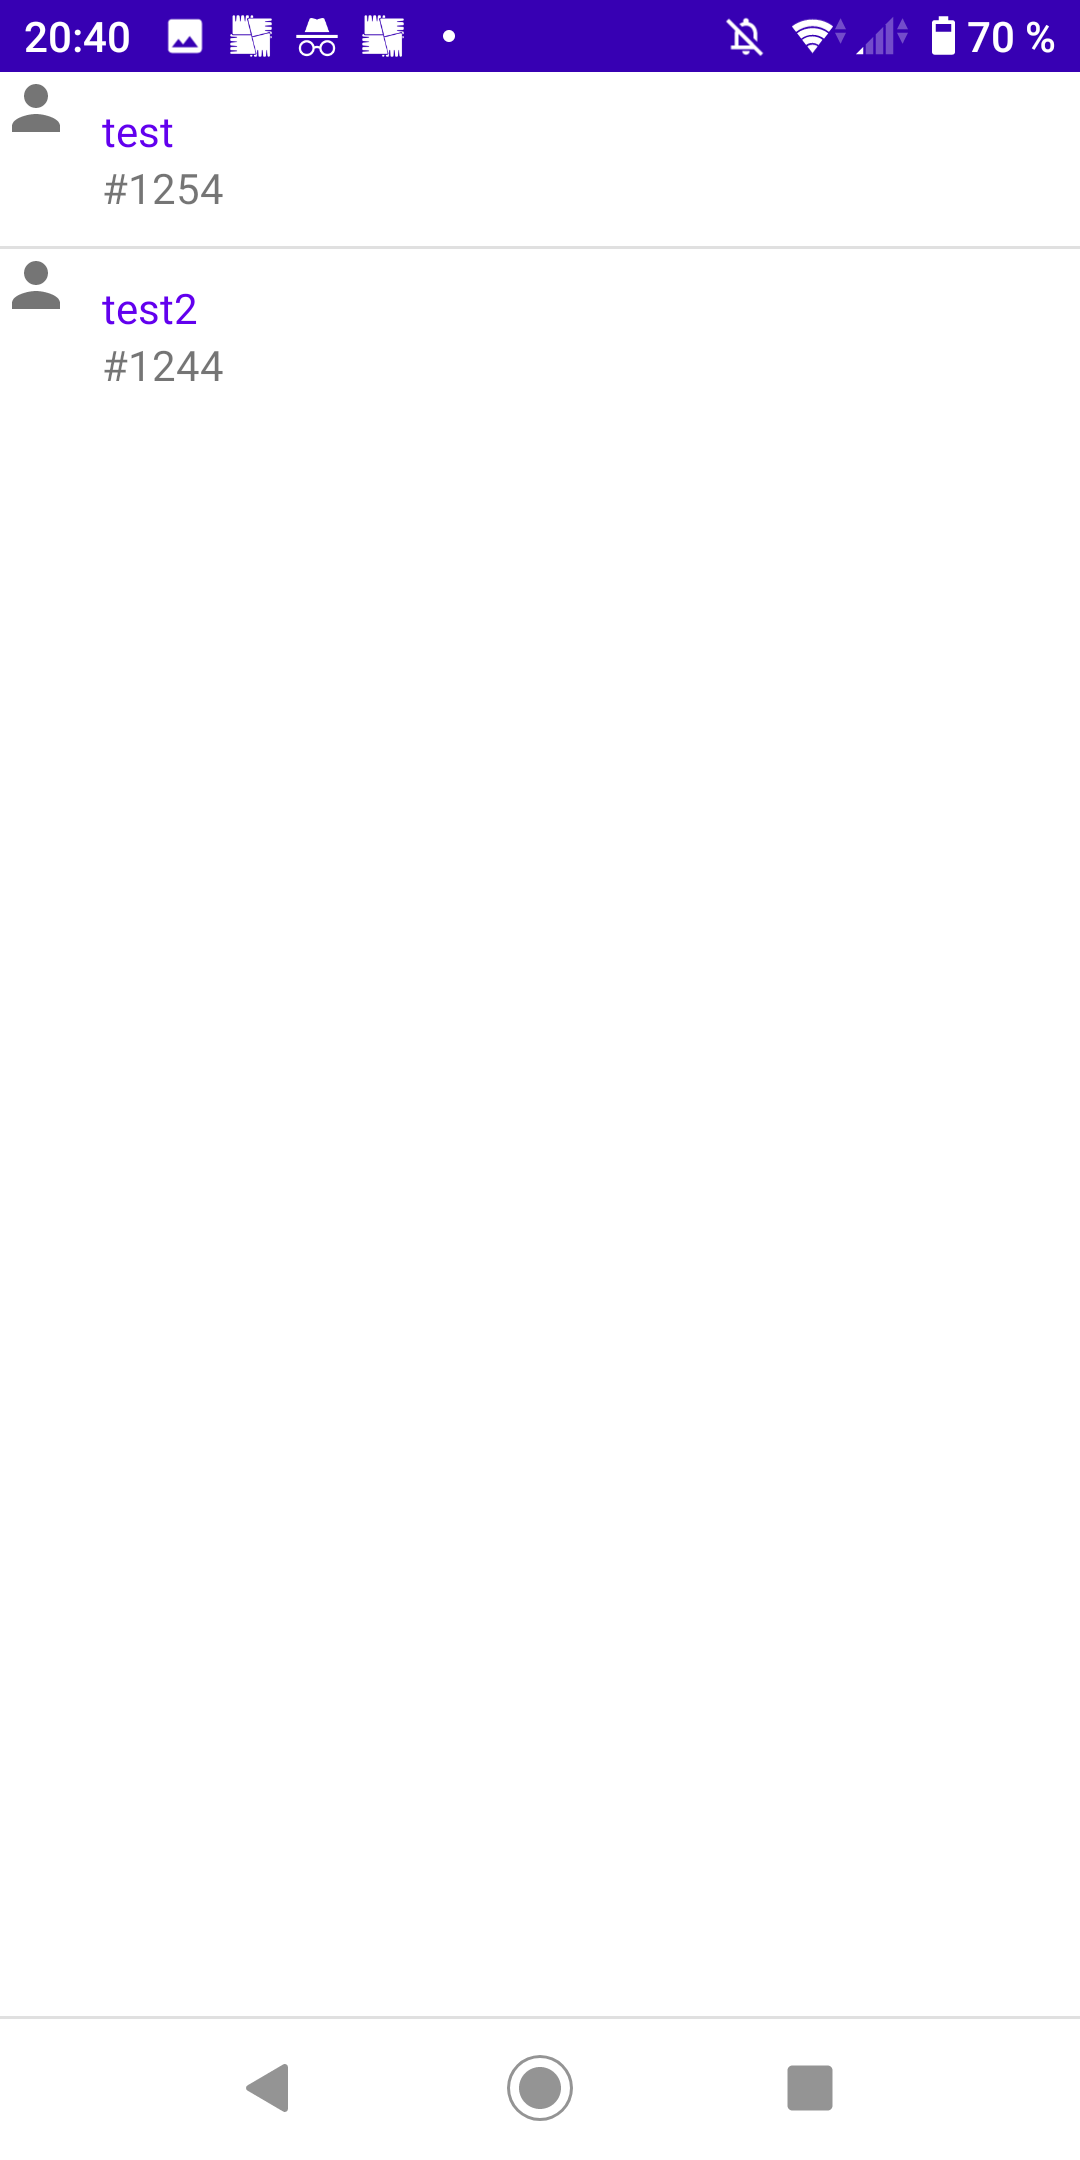
\includegraphics[width=5cm]{images/Contact_Page.png}
    \caption{Liste de Contacts.}
    \end{center}
    \end{figure}
    
Le menu permettant l'ajout de contact est accessible depuis la page principale par l'intermédiaire du bouton "Ajouter contact". Ce menu permet à l'utilisateur de saisir dans deux champs, le nom du contact qu'il souhaite ajouter ainsi que son id. Le bouton "sauvegarder" permet de sauvegarder ce contact dans une base sous forme de fichiers texte (.txt). Ce fichier permet de sauvegarder les contacts enregistrés dans l'application de manière permanente ainsi lorsque l'utilisateur quitte l'application ses contacts préférés ne sont pas effacés.
    \begin{figure}[H]
    \begin{center}
    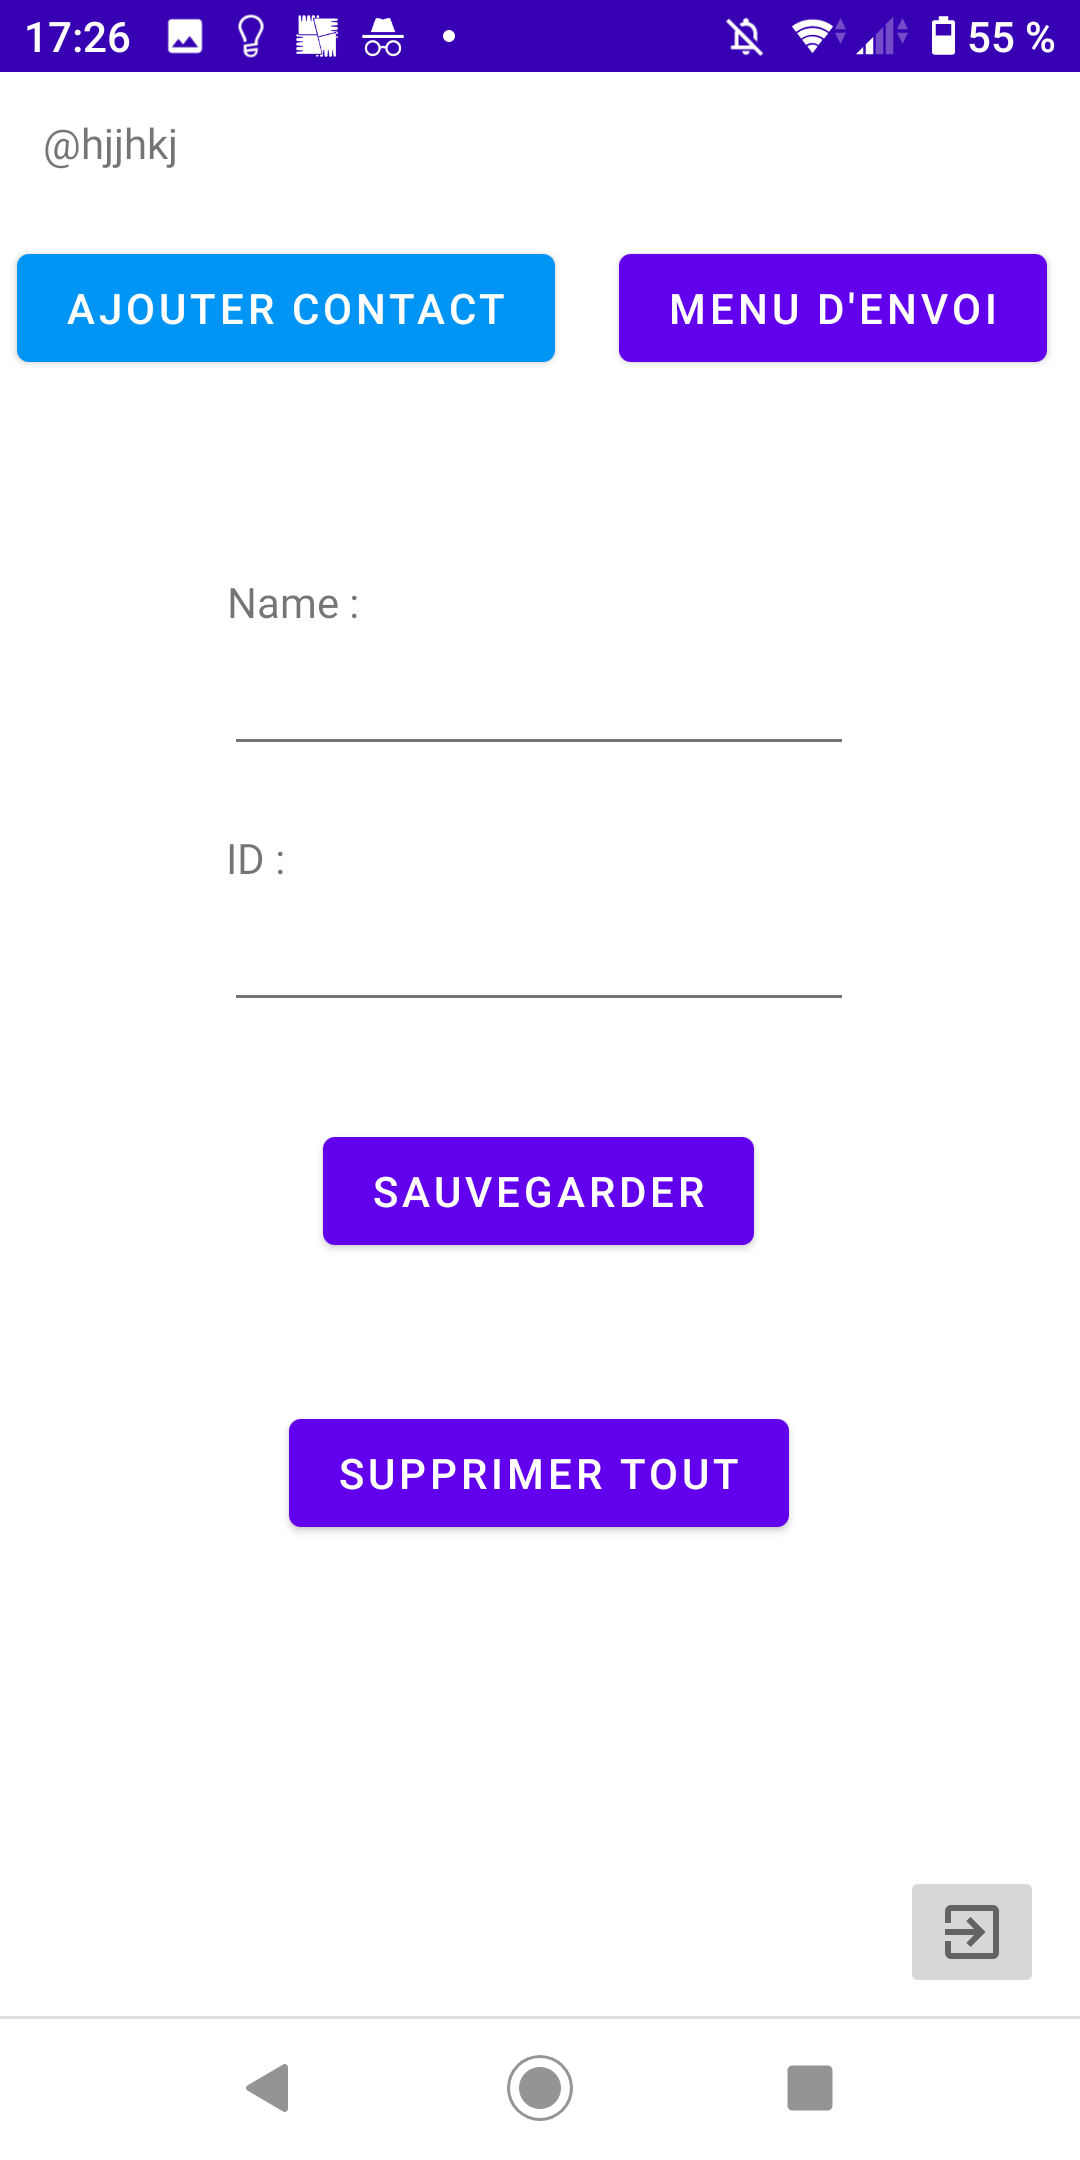
\includegraphics[width=7cm]{images/add_contact.png}
    \caption{Ajouter un Contact.}
    \end{center}
    \end{figure}
        
\chapter{ RÉALISATION }

        \section{Classes métier}
        Dans cette partie, nous allons décrire les classes les plus importantes dans le fonctionnement de l'application. Nous ne mentionnerons également que les méthodes les plus importantes de chaque classe.
        \begin{itemize}
        \vspace{0.2cm}
            \item \textbf{Client :} Cette classe permet de communiquer avec le serveur, elle est utile notamment pour l'inscription et la connexion au réseau Evernet. 
            \begin{lstlisting}[language = Java , frame = trBL , firstnumber = last , escapeinside={(*@}{@*)}]
            // Methodes de requetes serveur
            String signIn()
            HashMap<String, String> logIn()
            HashMap<String, String> getPhoneNb()
            HashMap<String,String> getPhoneNumList()
            String getInvitationKey()
            ArrayList<String> getAllAlias()
            
            // Communication
            openSocket()
            closeSocket()
            sendDataToServer()
            String receiveDataFromServer()
            
            // Parsing de donnees
            String truncateMarkers()
            String addMarkers()
            \end{lstlisting}
            
           \vspace{0.2cm}
            \item \textbf{Contact :} La classe Contact contient les informations des utilisateurs (nom et identifiant). Cette classe est Parcelable afin de permettre le passage d'un ArrayList d'objets de type Contact entre deux activités.
            \begin{lstlisting}[language = Java , frame = trBL , firstnumber = last , escapeinside={(*@}{@*)}]
            public void writeToParcel(Parcel dest, int flags);
            public Contact[] newArray(int size);
            
            \end{lstlisting}
            
             
            \item \textbf{Handler :} La classe Handler enregistre les différentes images (ReceivedFile) qu'elle reçoit.
            \vspace{0.2cm}
            
            \item \textbf{ContactAdapter :} Cette classe hérite de la classe BaseAdapter, elle a été conçue pour proposer un Adapter pouvant utilisée des objets de type Contact. Elle est utilisée dans la classe DisplayContact comme Adapter pour la Listview affichant les contacts à l'utilisateur.
            \vspace{0.4cm}
            
            \item \textbf{Packet :} la classe Packet décrit le format d'un paquet et permet de gérer les différents champs de ce dernier.
            \begin{lstlisting}[language = Java , frame = trBL , firstnumber = last , escapeinside={(*@}{@*)}]
            // Extraction des champs du paquet
             String extractSrc()
             String extractDst()
             String extractPosition()
             String extractNBpackets()
             String extractNameOfIm()
             String extractTtl()
             String extractFragment()
            \end{lstlisting}
            \vspace{0.2cm}
            
            \item \textbf{ReadWriteFile :}
            La classe ReadWriteFile permet l'écriture et la lecture de fichiers sur nos smartphones Android. Elle est principalement utilisée pour l'écriture et la lecture des certificats.
             \begin{lstlisting}[language = Java , frame = trBL , firstnumber = last , escapeinside={(*@}{@*)}]
            String readFromFile()
            String writeToFile()
            \end{lstlisting}
            \vspace{0.2cm}
            
            \item \textbf{SmsReceiver :} Cette classe permet de recevoir les SMS et les traiter en utilisant les classes Handler et ReceivedFile.
            \vspace{0.2cm}
           
            \begin{lstlisting}[language = Java , frame = trBL , firstnumber = last , escapeinside={(*@}{@*)}]     
            public View getView(int position, View convertView, ViewGroup parent)
            \end{lstlisting}
            \vspace{0.2cm}
            
            \item \textbf{FileManager :} Elle permet de compresser l'image et de la découper en fragments.
            \begin{lstlisting}[language = Java , frame = trBL , firstnumber = last , escapeinside={(*@}{@*)}]
            // Recupere une image stockee sur le telephone
            // et renvoie une bitmap compressee de l'image
            Bitmap getResizedBitmap()
            
            // Converti un entier en string et ajoute du bourrage si necessaire
            String intToString()
            
            // Recuperation du prochain fragment d'image donnee en String
            String getNextFragment()
            \end{lstlisting}
            \vspace{0.2cm}
            
            \item \textbf{ReceivedFile :} Elle permet à la réception, de regrouper les paquets ayant le même expéditeur et appartenant à la même image d'origine.\\
            Une fois que tous les paquets attendus sont reçus, elle concatène les fragments des paquets.  
            
            \begin{lstlisting}[language = Java , frame = trBL , firstnumber = last , escapeinside={(*@}{@*)}]
            insertPacket()
            
            // Conversion
            byte [] stringToArrayBytes()
            Bitmap byteArrayToBitmap()
            String toImageString()
            
            \end{lstlisting}
        \end{itemize}
        
        \section{Entête du paquet SMS }\label{epSMS}
        Pour fabriquer le paquet sms, nous nous sommes inspirés du format des paquets IP. Il comprend des champs qui permettent d'identifier sa source, sa destination, le fragment de l'image à envoyer, et d'autres éléments permettant la reconstruction de l'image à la réception des paquets. Les paquets ont le format ci-dessous : 
        
        \begin{table}[htbp]
          \begin{tabular}{|c|*{6}{c|}}
             \hline
             Source & Destination & Position & Nombre de paquets & Horodatage & TTL & Fragment  \\
             \hline
        \end{tabular} \\
        <--10---><------10-----><---8----><---------4--------------><-------6------><--1--><-------------
            \caption{Format d'un Paquet SMS}
            \label{tab:my_label}
        \end{table}
        
        \begin{itemize}
            \item \textbf{Source :} Correspond au pseudonyme  de l'expéditeur de l'image. Sa longueur est de dix caractères. \\
            \item \textbf{Destination :} Correspond au pseudonyme du destinataire final de l'image. Comme la source, la taille du champ destination est exactement de dix caractères. \\
            \item \textbf{Position :} C'est un tableau d'entiers qui correspond aux positions des fragments sur le nombre total de paquets. cette information permet d'ordonner les paquets à la réception.\\
            Le nombre de fragments contenus dans le paquet (c'est à dire ceux qui sont XOr) est égal au nombre d'entiers du tableau différents de zéro.\\
            \item \textbf{Nombre de paquets :} Ce champ correspond au nombre total de paquets obtenu après le découpage de l'image. Il permet de vérifier à chaque réception de paquet, si la totalité des paquets attendus a été reçu en comparant ce champs au nombre de paquets reçus.\\
            
            \item \textbf{Horodatage(timeStamp) :} Correspond à l'heure à laquelle l'image à envoyer a été découpée en fragments. Ce champ permet à la réception, d'éviter de mélanger des paquets qui, bien qu'ils proviennent de la même source, n'appartiendraient pas à la même image. Par exemple, un utilisateur peut envoyer simultanément deux images à quelqu'un, dans la mesure où les paquets empruntent différents chemins qui peuvent être plus ou moins  rapides. Un paquet de la seconde image peut arriver avant un paquet de la première. Dans ce cas, l'heure de découpage est le moyen que nous avons trouvé pour palier ce problème.\\
            Une image sélectionnée, découpée à 18heure 25 minutes 2 secondes aura pour timeStamp 182502. Cette technique a malgré tout sa limite. Par exemple un utilisateur envoie avec un téléphone tellement performant qu'il soit capable de sélectionner, découper, et envoyer les paquets de deux images différents dans un même temps. Un exemple typique serait que l'utilisateur découpe l'image nommée "A" à 18h25min02s et envoie tous les paquets, puis reprend la même procédure avec une deuxième image nommée "B" et qu'il soit toujours 18h25min02. Mais la probabilité que ce phénomène se produise est sensiblement très faible. Premièrement, nous n'avons pas parallélisé ces étapes, deuxièmement le nombre d'opérations qui s'effectuent dans les algorithmes de la sélection de l'image à l'envoi total des paquets est aussi grand.\\
            
            \item \textbf{TTL :} Comme pour les paquets IPs, ce champ correspond à la durée de vie d'un paquet. Il indique par combien d'intermédiaires le paquet pourra transiter avant qu'il arrive soit à la destination, ou qu'il soit détruit. C'est un entier qui se décrémente d'une unité à chaque intermédiaire.
            
            Dans notre projet, nous avons fixé sa valeur maximale à 9. Donc son champ occupe un caractère.\\
            \item \textbf{Fragment :} Fragment de l'image à envoyer. Comme indiqué dans la section ~\ref{decoupage}, la contrainte de la longueur maximale de caractères qui peuvent être envoyés d'un seul coup, nous oblige à limiter la longueur maximale d'un fragment à 100 caractères.
        \end{itemize} 
        
        
        \section{Algorithmes et méthodes}
         \subsection{Découpage de l'image}\label{decoupage}
        L'image à découper est transformée en tableau de pixels (bitmap), puis en tableau de bytes. 
        Les données à envoyer par SMS étant des chaînes de caractères, nous avons donc transformé ce tableau de bytes en une longue chaîne de caractères que nous avons par la suite découpée en petits fragments de chaînes de caractères de taille maximale 100. \\
        La longueur maximale d'un SMS ( paquet SMS dans ce projet) qui peut être envoyé d'un seul coup est de 160 caractères. Cette contrainte influe directement sur la longueur maximale des fragments de l'image et nous avons donc dû, pour faire de la place aux autres champs  de l'en-tête du paquet, limiter à 100 caractères la taille maximale d'un fragment.
        
        
        \paragraph{}
          Dans les champs source et destinataire, lorsque la longueur du pseudo est inférieure à 10, nous effectuons un bourrage avec le caractère "*".  Par exemple, le pseudo "Bob" devient "*******Bob" après bourrage.
          De même pour les paramètres position et nombre de paquets qui sont des entiers, nous bourrons avec des 0 au début. par exemple 3 et 15 deviennent respectivement 0003, 0015.
         \begin{lstlisting}[language = Java , frame = trBL , firstnumber = last , escapeinside={(*@}{@*)}]
         public Bitmap getResizedBitmap(ContentResolver cr, Uri u) throws IOException {
            originalImage = MediaStore.Images.Media.getBitmap(cr,u);

            width = originalImage.getWidth();

            height = originalImage.getHeight();
            matrix = new Matrix();
            scaleWidth = ((float) newWidth) / width;
            scaleHeight = ((float) newHeight) / height;
            matrix.postScale(scaleWidth, scaleHeight);
            resizedBitmap = Bitmap.createBitmap(originalImage, 0, 0, width, height, matrix, true);

            outputStream = new ByteArrayOutputStream();
            resizedBitmap.compress(Bitmap.CompressFormat.JPEG, 10, outputStream);
            imageBytes = outputStream.toByteArray();
            newWidth = resizedBitmap.getWidth();
            newHeight = resizedBitmap.getHeight();
            imageString = Base64.encodeToString(this.imageBytes, Base64.DEFAULT);
            Date currentTime = Calendar.getInstance().getTime();
            int heure = currentTime.getHours();
            int min = currentTime.getMinutes();
            int sec = currentTime.getSeconds();
            this.imageName = intToString(heure) + intToString(min) + intToString(sec);
         return resizedBitmap;
        }
        \end{lstlisting}
        %donner un exemple avec un shcema mettre la taille et le format des paquets
        
        \subsection{Gestion des paquets  par les noeuds à la réception}
        
        Lorsqu'un utilisateur reçoit un paquet, il vérifie dans l'en-tête s'il est le destinataire.\\
        \begin{itemize}
            \item  Si oui, alors il regarde dans sa hashmap s'il a déjà reçu des paquets du même expéditeur avec le même horodatage (timestamp). 
            \begin{itemize}
                     \item Si c'est le cas, alors il insère le paquet dans cette liste s'il n'y est pas.
                     \item Sinon il crée une nouvelle liste et l'insère pour dire que c'est le début d'une nouvelle image.
            \end{itemize}
            \item Sinon cela veut dire que ce paquet doit être transféré vers d'autres destinataires.
            Avant le transfert, il doit d'abord vérifier le TTL. S'il est supérieur à 1, alors il est décrémenté de 1, puis le paquet renvoyer à d'autres destinataires sélectionnés depuis le serveur. Nous avons implémenté deux versions dans le cas où le TTL est inférieur à 1 :
            \begin{itemize}
                \item On jette le paquet.
                \item On transfère le paquet directement à sa destination.
            \end{itemize}
        \end{itemize}
        La première version marcherait si le réseau était petit comme celui sur lequel nous réalisons les tests. Cependant, plus le réseau grandit, plus la probabilité que le destinataire finale fasse partie de la liste des prochains destinataires tirés du serveur devient petit. Donc, il se peut qu'aucun paquet n'arrive à destination.
        Finalement, nous avons gardé la deuxième version qui garanti l'envoi à la destination. \\
        
        La requête au serveur pour obtenir des destinataires intermédiaires ne renvoie rien si l'utilisateur a été déconnecté du serveur, donc pas authentifié. Dans ce cas, il doit se reconnecter et s'authentifier à nouveau avant de réessayer la requête. Si l'opération échoue toujours, alors le paquet est jeté.
        
        \begin{lstlisting}[language = Java , frame = trBL , firstnumber = last , escapeinside={(*@}{@*)},caption = Dans SmsReceiver]

    public void setPacketInHandler(Context context, String stringPack) {

        Packet packet=new Packet();
        packet.setPacket(stringPack);
        ReceivedFile file;
        String key=packet.getSource()+packet.getDestination()+packet.getTimeStamp();
        String myPhoneNumber=getDefaults(PHONE_NUMBER,context);
        if(packet.getDestination().equals(myPhoneNumber)) {
            boolean contains = handler.contains(key);
            if (contains==false) {
                file = new ReceivedFile(key);
                file.insertPacket(packet.getPosition(),packet.getImageFragment());
                file.setNbPackets(packet.getNbPackets());
                handler.insertFile(key,file);
            } else {
                file=handler.getFileByKey(key);
                file.insertPacket(packet.getPosition(),packet.getImageFragment());
            }
            Toast.makeText(context,"message :" + file.getSize(), Toast.LENGTH_LONG).show();
            this.imageView(context, file, key);
        } else {
            dashboardActivity = DashboardActivity.instance();
            packet.decreaseTTL();
            String target=null;
            if( packet.getTtl() <=1 ) {
                target= packet.getDestination();
            }
            dashboardActivity.sendTo(packet.getPacket(),target);
        }
    }

    \end{lstlisting}
          
         \subsection{Reconstitution et stockage de l'image à partir des paquets reçu}
         Après insertion d'un paquet, l'algorithme vérifie si tous les paquets attendus ont été reçus, en comparant le champ "Nombre de paquets" à la taille de la liste. Si les deux sont égaux, alors tous les paquets ont été reçus et dans ce cas on peut reconstruire l'image. 
        
        La reconstruction est l'opération inverse du découpage. On extrait le fragment d'image dans chaque paquet selon l'ordre croissant des numéros des paquets (de 0 à Nombre de paquets - 1), puis on concatène ces fragments pour former une longue chaîne de caractères.\\
        
        Cette chaîne  est ensuite transformée  en un tableau de bytes (arrayBytes) et enfin tableau de pixels(bitmap). L'utilisateur recevra une notification "Image reçue". \\
         Pour l'instant nous sauvegardons les images que nous recevons de l'application dans la galerie, dans un dossier appelé "Pictures" avec comme nom PSEUDO + timestamp. Les images dans ce dossier se classent de la plus récente à la plus anciennement reçue. Ce qui permet à l'utilisateur de retrouver plus facilement les images reçue tout dernièrement.\\
       
       \begin{lstlisting}[language = Java,frame = trBL , firstnumber = last , escapeinside={(*@}{@*)}, caption=Dans SmsReceiver.java ]
            public void imageView(Context context, ReceivedFile file, String key) {

                if(file.allPacketReceived()) {
                        byte [] bytes = file.stringToArrayBytes();
                        Toast.makeText(context,"Image recue :" + bytes.length, Toast.LENGTH_LONG).show();
                        Bitmap bitmap = file.byteArrayToBitmap(bytes);
                        MediaStore.Images.Media.insertImage(context.getContentResolver(), bitmap, key, "EvernetImage");
                }
            }
       \end{lstlisting}
      
        \subsection{Network Coding Topologie}
        
            Dans un premier temps et dans le but d'avancer dans le projet, nous a décidé de fixer la topologie dans laquelle s'insère le Network Coding, et pour cela, on l'a adaptée pour avoir une destination, une source et quatre nœuds intermédiaires. D’abord, la topologie est fixée dans la source après avoir demandé au serveur quatre nœuds intermédiaires. Ensuite, la topologie sera envoyée au serveur pour qu’elle soit exploitée quand un nœud intermédiaire demande une liste de destinataires. Quand un nœud intermédiaire reçoit deux paquets différents et c’est lui le responsable de l’encodage, il encode immédiatement, ce sont deux derniers et il envoie le paquet encoder à son voisin renvoyé par le serveur. Enfin, une fois que la destination a reçu tous les paquets soit encodée ou non elle procède pour le décodage des paquets encodés en utilisant les paquets en clair (non chiffrés).
        
        \begin{figure}[H]
                \centering
                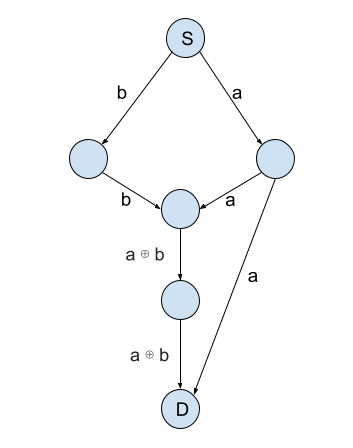
\includegraphics[scale=0.5]{images/NC_topology.png}
                \caption{Topologie Network Coding réaliser}
                \label{fig:Network_Coding_Topologie}
        \end{figure}
        
        \subsection{Network Coding implémentation}
        
        \paragraph{} Le Network Coding est un point capital de cette application. Cette notion de Network Coding étant nouvelle, nous avons pris du temps pour effectuer des recherches et comprendre comment l'appliquer dans notre projet. La difficulté ici est la particularité du réseau. En effet dans les exemple que l'on a pu voir au sujet du Network Coding, les noeuds du réseau peuvent physiquement communiquer avec leurs voisins.
        Le réseau sur lequel nous travaillons n'ayant pas de voisin physique, fixer une topologie comme celle vue précédemment est nécessaire.
        Une nécessité que nous n'avons compris que très tard. Cela a fortement impacté l'avancement de notre projet.\\
        Nous avons essayé d'implémenter deux versions du Network Coding. À ce jour aucune de ces implémentations n'a pu êtres testées.
        
        
        \subsubsection{Implémentation élimination de Gauss-Jordan}
        
        \paragraph{}La première implémentation consiste à encoder les fragments des paquets en une combinaison linéaire.
        Une combinaison linéaire de la forme : \textbf{Ax + By}, \textbf{A} et \textbf{B} étant les fragments et \textbf{x}, \textbf{y} leurs coefficients respectifs.
        Le nouveau fragment créé est ainsi envoyé au noeud suivant pour y être combiné à nouveau dans le cas d'un noeud intermédiaire, ou bien d'être décodé s'il s'agit de la destination.
        
        \paragraph{}Il existe plusieurs méthodes pour résoudre un système d'équations linéaires.\\
        Dans le cas du Network Coding la solution la plus adaptée est l'élimination de Gauss-Jordan. 
        Pour ce faire on crée une matrice de taille n*n, "n" étant le nombre de fragment d'une image. 
        On a donc chaque colonne de la matrice qui correspond à un fragment de l'image.
        Chaque ligne de la matrice correspondant à une combinaison linéaire de ces fragments.
        Les nombres dans la matrice représentent donc les coefficients attribués aux fragments dans les combinaisons linéaires.
        En parallèle on construit un vecteur colonne de taille n, avec les valeurs des fragments en faisant correspondre les valeurs des lignes du vecteur avec les combinaisons des lignes de la matrice.
        Pour simplifier le développement nous nous sommes appuyés sur une la librairie \textbf{"la4j"}\cite{la4j}.
        Cette librairie dispose d'une fonction solve().
        Cette fonction est appelée sur la matrice précédemment créée en passant en argument le vecteur colonne contenant les valeurs de fragments.\\
        Nous avons cependant rencontré un problème au niveau des types entre les valeurs des paquets qui sont de type "long" et les valeurs dans la matrice qui sont elles des "double".
        La conversion "long" vers "double" fait perdre des chiffres, ce qui fausse la résolution du système d'équation. 
        On obtient donc un résultat erroné.\\
        
        \paragraph{}Pour résoudre ce problème il faudrait écrire des fonctions adapté à notre format. La Dead-Line se rapprochant nous avons choisi d'implémenter une version simple de Network Coding. Cela afin d'avoir un modèle à présenter.
        
        \subsubsection{Implémentation XOR}
        
        L'utilisation du XOR pour le Network Coding permet de visualiser de façon simple le but et l'intérêt du NC.
        Dans la topologie vu précédemment sur le schéma figure : \ref{fig:Network_Coding_Topologie}  , si un paquet arrive sur un noeud relais alors celui-ci l'encode avec le prochain paquet de la même image qu'il recevra.\\
        Quand un appareil reçoit un paquet encodé, il regarde s'il peut le décoder avec les paquets déjà reçus.
        Si ce n'est pas possible il le stock pour le déchiffré si possible avec le prochain paquet reçus.
        L'encodage et le décodage se font à l'aide de l'opération binaire XOR.\\
        
        Fonction d'encodage des fragments :
        
        \begin{lstlisting}[language = Java , frame = trBL , firstnumber = last , escapeinside={(*@}{@*)}]
        
        static public Packet mergeTwoPackets(Packet firstPacket, Packet secondPacket){

            String firstPacketFragment = firstPacket.getImageFragment();
            String secondPacketFragemnt =  secondPacket.getImageFragment();
    
            int[] firstPacketPos = firstPacket.getPosition();
            int[] secondPacketPos = secondPacket.getPosition();
    
            int[] mergePacketPos = {firstPacketPos[0],secondPacketPos[0]};
    
            byte[] firstPacketFragmentBytes = firstPacketFragment.getBytes();
            byte[] secondPacketFragmentBytes = secondPacketFragemnt.getBytes();
    
            byte[] mergedPacketsFragmentBytes = new byte[firstPacketFragmentBytes.length];
    
            for (int i=0; i < mergedPacketsFragmentBytes.length; i++){
                mergedPacketsFragmentBytes[i] = (byte) (firstPacketFragmentBytes[i] ^ secondPacketFragmentBytes[i]);
            }
    
            String mergedPacketsFragment = new String(mergedPacketsFragmentBytes);
    
    
    
            Packet output = new Packet(firstPacket.getSource(),
                    firstPacket.getDestination(),
                    mergePacketPos,
                    firstPacket.getNbPackets(),
                    firstPacket.getTtl(),
                    firstPacket.getTimeStamp(),
                    mergedPacketsFragment);
            return output;
        }
        
        \end{lstlisting}
        \\
        
        Fonction de décodage des des Fragments :
        
        \begin{lstlisting}[language = Java , frame = trBL , firstnumber = last , escapeinside={(*@}{@*)}]
        
        static public Packet decodeMergedPacketWithOnePacket(Packet mergedPacket, Packet complementaryPacket){

            String mergedPacketFragment = mergedPacket.getImageFragment();
            String complementPacketFragment = complementaryPacket.getImageFragment();
    
            byte[] mergedPacketFragmentBytes = mergedPacketFragment.getBytes();
            byte[] complementPacketFragmentBytes = complementPacketFragment.getBytes();
    
            byte[] decodedPacketFragmentBytes = new byte[mergedPacketFragmentBytes.length];
    
            for (int i=0; i < mergedPacketFragmentBytes.length; i++){
                decodedPacketFragmentBytes[i] = (byte) (mergedPacketFragmentBytes[i] ^ complementPacketFragmentBytes[i]);
            }
    
            int[] mergedPacketPos = mergedPacket.getPosition();
            int[] complementPacketPos = complementaryPacket.getPosition();
    
    
    
            int[] decodedPacketPos = {complementPosInMerged(mergedPacketPos,complementPacketPos[0])};
            String decodedPacketFragment = new String(decodedPacketFragmentBytes);
    
            Packet decodedPacket = new Packet(complementaryPacket.getSource(),
                    complementaryPacket.getDestination(),
                    decodedPacketPos,
                    complementaryPacket.getNbPackets(),
                    complementaryPacket.getTtl(),
                    complementaryPacket.getTimeStamp(),
                    decodedPacketFragment);
    
            return decodedPacket;
    }
        
        \end{lstlisting}
 
\chapter{ TESTS}
Dans cette section nous présentons les tests unitaires et d'intégration réalisés sur les classes implémentées dans la partie Modèle. Dû à une contrainte de temps, nous n'avons pas pu réaliser de tests automatiques dit "end to end".  Nous avons tout de même testé manuellement les différentes fonctionnalités liées à l'interface, bien que cela ne soit pas suffisent.
\\
Les tests ont été lancés depuis Android studio en utilisant JUnit (version min 4.+). 

\subsection{Test classe FileManager}
La classe FileManager ne nécessite pas de beaucoup de tests unitaires puisqu'elle fait majoritairement appel à des fonctions liées à l'API Android (Bitmap, Matrix). 
Par conséquent nous avons eu besoin de tester les méthodes intToString, et getNextFragment.
Il est nécessaire de s'assurer du bon retour de getNextFragment puisque c'est grâce à cette méthode que l'on peut envoyer chaque partie de l'image, cela joue donc un rôle clé dans la futur reconstruction.

\begin{figure}[H]
    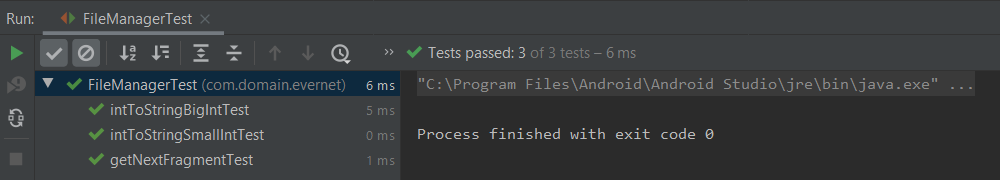
\includegraphics[width=18cm]{images/fileManagerOutput.png}
    \caption{Sortie de la classe de test FileManager.}
\end{figure}

\subsection{Test classe Client}
La classe Client joue un des rôles majeurs dans l'application Evernet, il est nécessaire de s'assurer de son bon fonctionnement. Nous avons donc testé la communication avec le serveur du groupe 1, c'est à dire l'ouverture, et la fermeture de sockets, ainsi que l'envoi et la réception de données. Il s'agit donc de la seule classe qui bénéficie de tests d'intégration puisque les tests font appel à la bibliothèque Java Socket qui n'est pas "mock".
\\
Cette classe nous a demandé le plus de travail en temps, puisque les tests d'intégration sont plus délicats à réaliser, en effet nous n'avons pas la main sur le serveur et la base de données, ce qui complexifie le processus. Nous avons donc réalisé ces tests avec le groupe 1 qui s'est tenu disponible pour nous aider à débugger lorsque nécessaire.
\\
\\
Deux tests unitaires sont réalisés permettant d'une part de vérifier le découpage correcte des réponses du serveur pour retirer les marqueurs de début et de fin, et d'autre part la construction d'une requête avec les marqueurs.
\begin{figure}[H]
    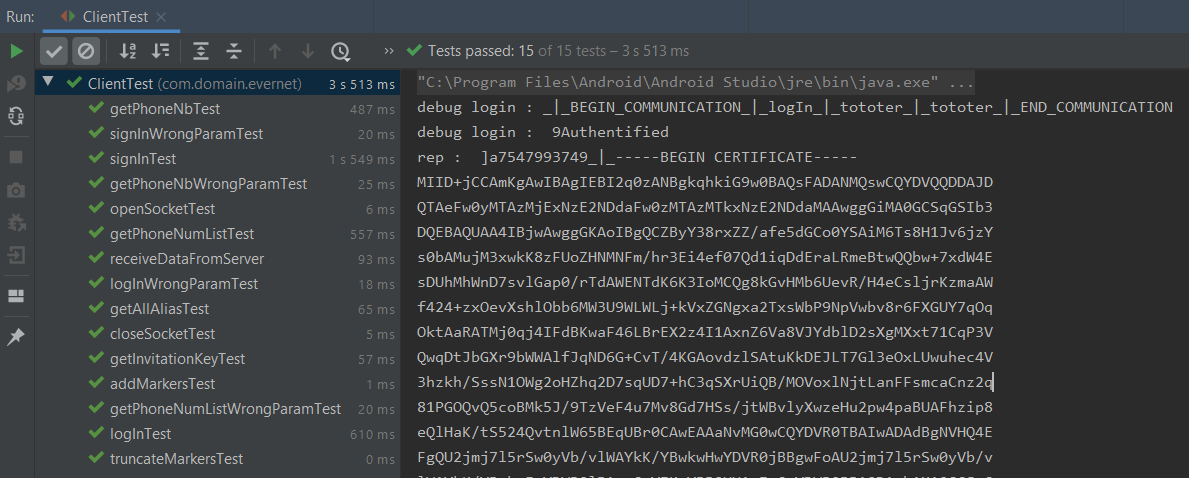
\includegraphics[width=18cm]{images/clientTestOutput.png}
    \caption{Sortie de la classe de test Packet.}
\end{figure}



\subsection{Test classe Packet}
La classe paquet est une autre classe majeure puisqu'elle joue un rôle clé dans le fonctionnement global du network coding. Il est donc très important de s'assurer que l'extraction de chaque champs d'un paquet est correctement réalisé. Nous avons également testé notre méthode permettant de générer un bourrage sur les champs concernés.

\begin{figure}[H]
    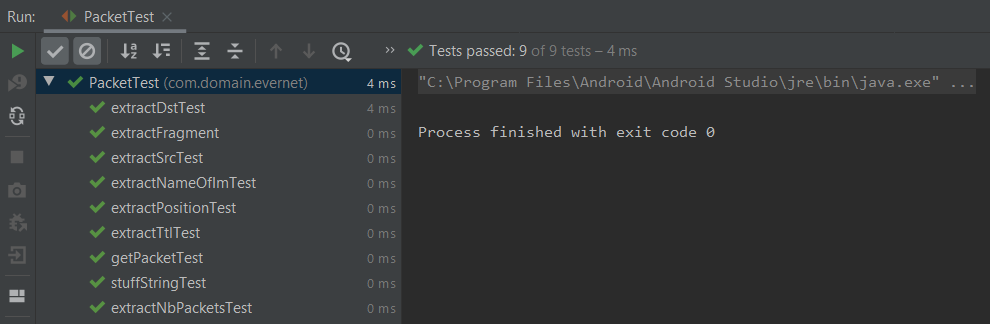
\includegraphics[width=18cm]{images/packetTestOutput.png}
    \caption{Sortie de la classe de test Packet.}
\end{figure}

\chapter{ CONCLUSION}
%ce qui a été réussi, ce qui n'a pas été et les perspectives
% les apports du projet 
{La réalisation de ce projet  de fin d'études nous a permis :
\begin{itemize}
    \item de revoir les concepts principaux du génie logiciel et de les remettre en application : besoins fonctionnels et non fonctionnels, conception et spécification, tests, architecture et modularité, outils d'aide au développement, travail en équipe.
    \item de renforcer nos connaissances en programmation : paradigmes de programmation, langages de programmation, gestion des erreurs.
    \item d'appliquer une pratique scientifique rigoureuse en développement logiciel : recherche et analyse de l'existant, bibliographie, assimilation de nouveaux concepts, justification des choix, analyses et critiques du travail réalisé, rédaction de documents(Compte rendu hebdomadaire, cahier des besoins, rapport final et présentations).
    \item de découvrir et d'utiliser le célèbre système d'exploitation Android pour développer une application mobile.
    \end{itemize}{}\par}
{Malgré des conditions difficiles de réalisation du projet liées au temps que nous disposions pour ce dernier, à la fermeture de l'université et au contraintes matérielles (pour les tests par exemple), nous avons dans un premier temps essayer d'obtenir sans le network coding un outil qui traite les besoins essentiels du client :
    \begin{itemize}
        \item sélectionner une image et un destinataire 
        \item la découper en plusieurs slots 
        \item envoyer les slots à des intermédiaires qui les enverront directement au destinataire
        \item  Reconstituer l'image à la réception de tous les slots
    \end{itemize}{}\par}

Pour la mise en place du Network coding nous avons réussi : 
 \begin{itemize}
        \item l'opération d'encodage et de décodage avec un XOR : on a réussi au niveau d'un noeud à encoder deux paquets et à décoder le packet formé pour retrouver les paquets d'origine. 
        \item le traitement des paquets par le destinataire : cette étape n'a pas été testé sur le réseau physique. 
    \end{itemize}

L'encodage et le décodage en utilisant les combinaisons linéaires n'est pas encore fonctionnel et il reste à intégrer le network coding lors du traitement des paquets au niveau des noeuds intermédiaires.
    
    
    \vspace{0.2cm}
    Des améliorations qui seraient importantes à implémenter pour un futur travail seraient d'une part de chiffrer nos SMS pour assurer la confidentialité des données transitant dans le réseau Evernet; d'autre part il serait intéressant de pouvoir faire un multicast de l'envoi d'une image.
    
    \vspace{0.2cm}
    Nous ne saurons terminer ce rapport sans remercier toutes les personnes qui, de près ou de loin ont contribué à la réalisation de ce projet. Nous pensons en particulier au professeur chargé du cours de MOCPI \textbf{Monsieur Pascal DESBARATS} pour son encadrement et ses conseils et au client \textbf{Monsieur Serge CHAUMETTE} pour sa disponibilité et son implication tout au long du processus.


\printbibliography
\end{document}